
\section{Mise en contexte}

\subsection{Introduction}

Les routes réduisent la continuité écologique des milieux et constituent un obstacle physique et biologique à la faune et à la flore \citep{forman1998}. Lorsqu'une route est créée, cette nouvelle barrière peut réduire l'abondance d'une population en augmentant la mortalité \citep{seiler2020,rytwinski2016}. Plusieurs milliards d'animaux sont tués annuellement sur les routes, et la majorité des études ciblent sur les carnivores et les ongulés \citep{barrientos2021}. Pourtant, la traversée des routes est d'autant plus dangereuse pour la faune qui n'a pas une grande capacité de déplacement, et qui emprunte le même chemin pour rejoindre différents habitats chaque année \citep{gunson2019, jones2022, langen2009}. À long terme, cette fragmentation due aux routes affectera le maintien de certaines populations animales et végétales \citep{gonzalezgallina2013}.  
Au Canada, peu de passages fauniques sont spécifiquement conçus pour l'herpétofaune. Les rares projets de recherche sur ces taxons ont été réalisés sur des routes secondaires avec des passages de petits diamètres \citep{retamal2020}, ce qui n'est pas représentatif du paysage routier global. Pourtant, de nombreuses espèces souffrent d'une perte de connectivité imputable à la fragmentation du paysage, en partie lié à la multiplication des routes. C'est le cas de la rainette faux-grillon (Pseudacris triseriata) de la région de la Montérégie au Québec, qui a été désignée menacée selon la Loi sur les espèces en péril du Canada \citep{cosepac2008} et la Loi sur les espèces menacées ou vulnérables (L.R.Q., c. E-12.01). La tortue serpentine (Chelydra serpentina), tout comme la tortue peinte du Centre (Chrysemys picta marginata) et la tortue peinte de l’Est (Chrysemys picta picta) sont désignées par la Loi sur les espèces en péril du Canada comme espèces préoccupantes à l’Annexe 1.
L'objectif de ce projet vise à combler les lacunes sur les critères favorisant la connectivité écologique de la petite faune. Les résultats de ces travaux de recherche serviront à la planification d'autres projets à long terme, appliquant la méthodologie Before-After Control-Impact (BACI) aux passages adaptés à l'herpétofaune \citep{jones2022}.

\subsection{Changement d'orientation du projet de recherche}

Un premier livrable du projet de recherche R875.1 a été remis en juin 2024. Durant la rencontre de suivi 1 en septembre 2024, le ministère des Transports et de la Mobilité durable (MTMD) a annoncé que le calendrier des aménagements de passages fauniques sur l’Autoroute 10 (A10) et la Route 104 (R104) étaient reportés sans date fixe pour la prévision des travaux sur ces deux axes routiers. Les travaux du MTMD devaient consister à : (1) élargir les chaussées afin de fluidifier le trafic et de réduire la congestion automobile aux heures de pointe, tout en encourageant l’utilisation des transports en commun et le covoiturage; (2) remplacer et modifier certains ponceaux pour les aménager en passages fauniques spécifiques à l’herpétofaune. L'équipe du laboratoire de recherche en biologie de la conservation quantitative de l'Université Laval a été mandatée pour inventorier et suivre l'herpétofaune en amont et en aval des travaux. En l’absence de date prévue pour la construction des passages fauniques sur l’A10 et la R104, l’équipe de recherche a proposé un avenant au projet afin de réorienter les objectifs initiaux en fonction de ces nouvelles contraintes. Cet avenant a été approuvé par l’ensemble des parties le 21 mai 2025. Le budget du projet de recherche est inchangé, seuls les objectifs ont été modifiés. 

\begin{figure}[H]
\centering
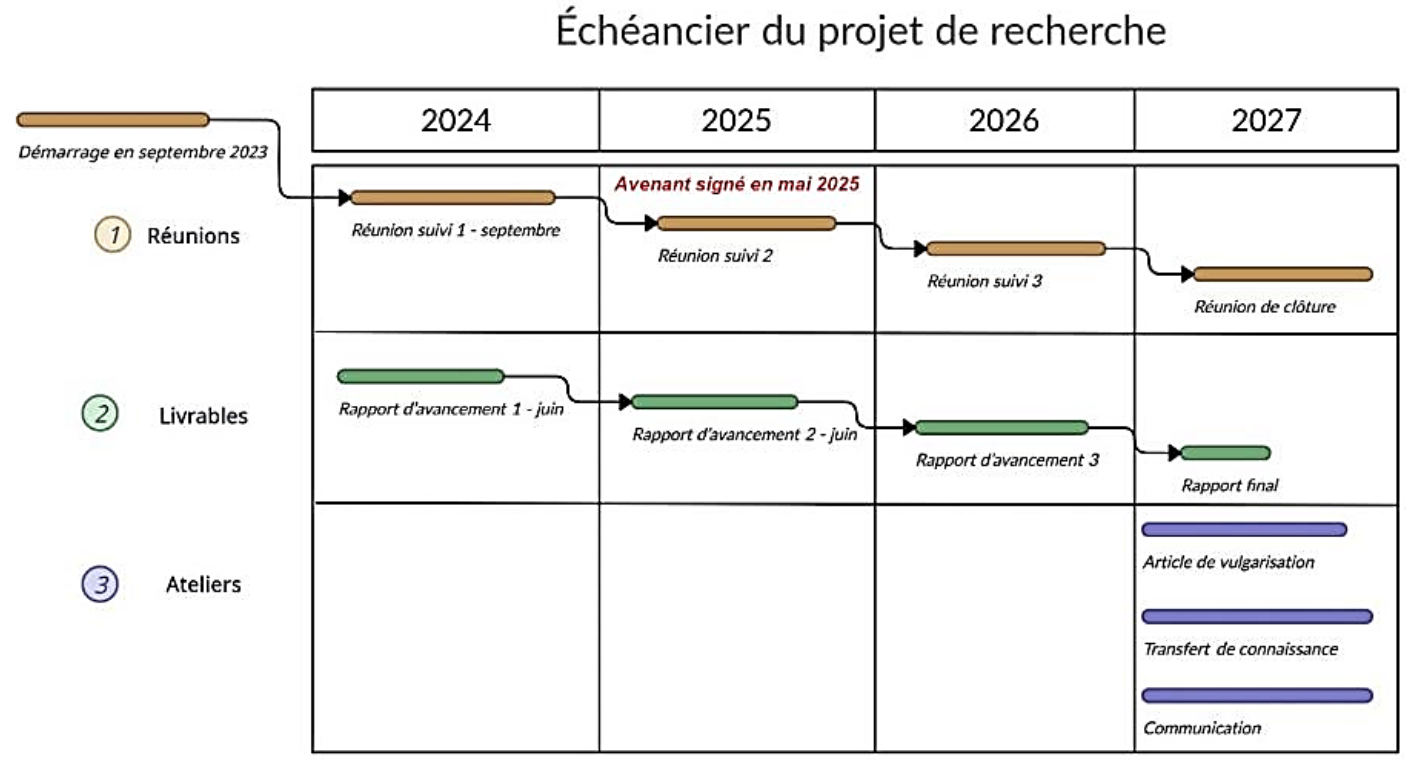
\includegraphics[width=0.8\textwidth]{figs_monteregie_liv3/echeancier.png}
\caption{Échéancier du projet de recherche entre 2023 et 2027. L'avenant 1 du
contrat R875.1 a été signé en mai 2025.}
\label{fig:echeancier26}
\end{figure}

Suite à ces changements, le deuxième livrable fut compartimenté en deux parties. Une partie était dédiée aux passages fauniques sur l'A10 et la 104. Une deuxième partie était dédiée à l'évaluation des critères de connectivité écologique. Par conséquent, le troisième et quatrième livrables suivront la même trâme afin de rendre compte des différents volets.

Dans ce troisième livrable, nous présentons les dernières avancées en matière d'échantillonnage et d'analyse des fichiers numériques, soit les images des pièges photographiques et les enregistrements des Audiomoths. Bien que nous y dressions un portrait détaillé des résultats obtenus à ce jour, ce rapport ne comporte pas d'analyses statistiques avancées. Celles-ci seront présentées dans le dernier livrable, une fois la compilation des derniers résultats finalisée pour 2026 et les derniers fichiers numériques analysés.

Nous ne reviendrons pas sur les résultats de terrain de 2024, déjà traités dans le livrable précédent. Dans la partie II, nous exposons les résultats issus de l'analyse par MegaDetector de l'ensemble des images captées par les pièges photographiques installés sur l'A10 et la 104 en 2024. Nous présentons ensuite les derniers résultats obtenus en 2025 pour les suivis de mortalité ainsi que pour les inventaires des milieux humides et de la petite faune, auxquels s'ajoutent les analyses des images des pièges photographiques déployés dans 18 ponceaux en 2025, soit 54\% des images récoltées cette année-là. L'échéancier présenté à la Fig.~\ref{fig:echeancier26} illustre les prochaines étapes du projet. 

À la suite de chaque dépôt de rapport, le comité aura l’occasion de lire et de commenter le document. Le comité de suivi se réunira pour une présentation du présent rapport par l'équipe de recherche, et les membres du comité pourront fournir des commentaires, demander des précisions, ou formuler des recommandations pour la suite. Enfin, une fois le rapport final du projet déposé et la réunion de clôture terminée, une activité de transfert technologique pourra être proposée sous forme d'atelier ou de colloque en invitant différents partenaires des milieux municipaux, gouvernementaux et académiques.
